\documentclass[]{article}
\usepackage{geometry}
\geometry{a4paper, left=20mm, top=20mm,}
\usepackage{graphicx}
\usepackage{float}
\usepackage{hyperref}
\usepackage{booktabs}
\usepackage{amsmath}
\usepackage{units}
\usepackage{cleveref}

\usepackage{longtable}

\newcommand{\iftab}{\fontshape{sl}\selectfont}

\newcommand{\bftab}{\fontseries{b}\selectfont}

\begin{document}

\section*{Software Information}

\begin{itemize}
\item Please check, whether your inputs, the equations applied and the charactersitics are displayed correctly.
\item You are welcome to send your feedback via \url{https://github.com/oemof/tespy/issues}.
\item \LaTeX packages required are:
\begin{itemize}
\item graphicx
\item float
\item hyperref
\item booktabs
\item amsmath
\item units
\item cleveref
\item longtable
\end{itemize}
Additionally, you will need to make the following definitions:
\begin{itemize}
\item \textbackslash newcommand\{\textbackslash iftab\}\{\textbackslash fontshape\{sl\}\textbackslash selectfont\}
\item \textbackslash newcommand\{\textbackslash bftab\}\{\textbackslash fontseries\{b\}\textbackslash selectfont\}
\end{itemize}
\item To suppress these messages, call the model documentation with the keyword draft=False in the formatting dict.
\end{itemize}

\begin{table}[H]
\begin{tabular}{ll}
\bftab General information&\\
& \\
TESPy Version:&0.5.0 - Davis' Domain\\
Commit:&70bf8da9@dev\\
CoolProp version:&6.4.0\\
Python version:&3.7.6 (default, Jan  8 2020, 20:23:39) [MSC v.1916 64 bit (AMD64)]\\
Documentation generated:&Oktober 06, 2021\\
& \\
\bftab Parameter highlighting&\\
& \\
Variable component parameters:& \iftab italic\\
Specified input parameter:& \bftab bold\\
Results of simulation:& normalfont \\
& \\
\multicolumn{2}{l}{\iftab Equations are displayed for input parameters only.}\\
\end{tabular}
\end{table}
\newpage\section{Connections in offdesign mode}

\subsection{Connection specifications and results}

\begin{table}[H]
\centering
\caption{Connection specifications and results}
\begin{tabular}{lrrrrr}
\toprule
{} & m in $\unitfrac[]{kg}{s}$ & p in $\unit[]{bar}$ (\ref{eq:Connection_pressure}) & h in $\unitfrac[]{kJ}{kg}$ & T in $\unit[]{^\circ C}$ (\ref{eq:Connection_temperature}) & s in $\unitfrac[]{J}{kgK}$ \\
label                                                          &                           &                                                    &                            &                                                            &                            \\
\midrule
ambient air:out1\_compressor:in1                               &                   593.342 &                                       \bftab 1.000 &                    293.562 &                                                \bftab 20.0 &                   7,008.57 \\
compressor:out1\_combustion:in1                                &                   593.342 &                                             15.000 &                    697.245 &                                                      411.2 &                   7,100.93 \\
fuel source:out1\_fuel compressor:in1                          &                    14.341 &                                              1.000 &                    882.999 &                                                       20.0 &                   6,565.56 \\
fuel compressor:out1\_combustion:in2                           &                    14.341 &                                             15.000 &                  1,522.678 &                                                      272.4 &                   6,746.87 \\
combustion:out1\_gas turbine:in1                               &                   607.683 &                                             15.000 &                  1,965.585 &                                                    1,319.0 &                   8,118.17 \\
gas turbine:out1\_superheater:in1                              &                   607.683 &                                              1.051 &                  1,132.594 &                                                      657.2 &                   8,222.06 \\
superheater:out1\_evaporator:in1                               &                   607.683 &                                              1.041 &                    970.315 &                                                      519.3 &                   8,036.29 \\
evaporator:out1\_economizer:in1                                &                   607.683 &                                              1.030 &                    780.728 &                                                      352.4 &                   7,770.80 \\
economizer:out1\_chimney:in1                                   &                   607.683 &                                       \bftab 1.020 &                    552.018 &                                               \bftab 142.0 &                   7,328.77 \\
economizer:out2\_drum:in1                                      &                   102.457 &                                            132.653 &                  1,531.848 &                                                      331.0 &                   3,560.66 \\
drum:out1\_evaporator:in2                                      &                   409.828 &                                            132.653 &                  1,542.018 &                                                      332.4 &                   3,577.47 \\
evaporator:out2\_drum:in2                                      &                   409.828 &                                            132.653 &                  1,823.132 &                                                      332.4 &                   4,041.67 \\
drum:out2\_superheater:in2                                     &                   102.457 &                                            132.653 &                  2,656.304 &                                                      332.4 &                   5,417.50 \\
superheater:out2\_ls sink:in1                                  &                   102.457 &                                     \bftab 130.000 &                  3,618.800 &                                                      607.2 &                   6,781.95 \\
ls source:out1\_steam turbine high pressure:in1                &                   102.457 &                                            130.000 &                  3,618.800 &                                                      607.2 &                   6,781.95 \\
steam turbine high pressure:out1\_mp split:in1                 &                   102.457 &                                              0.360 &                  2,468.707 &                                                       73.3 &                   7,234.60 \\
mp split:out1\_district heating condenser:in1                  &                     4.624 &                                              0.360 &                  2,468.707 &                                                       73.3 &                   7,234.60 \\
district heating condenser:out1\_feed water pump 1:in1         &                     4.624 &                                              0.356 &                    306.027 &                                                       73.1 &                     992.72 \\
feed water pump 1:out1\_merge:in1                              &                     4.624 &                                            132.653 &                    447.111 &                                                      104.3 &                   1,345.13 \\
mp split:out2\_mp valve:in1                                    &                    97.833 &                                              0.360 &                  2,468.707 &                                                       73.3 &                   7,234.60 \\
mp valve:out1\_steam turbine low pressure:in1                  &                    97.833 &                                              0.360 &                  2,468.707 &                                                       73.3 &                   7,234.60 \\
steam turbine low pressure:out1\_condenser:in1                 &                    97.833 &                                              0.056 &                  2,250.125 &                                                       35.0 &                   7,331.32 \\
condenser:out1\_feed water pump 2:in1                          &                    97.833 &                                              0.056 &                    145.875 &                                                       34.8 &                     502.67 \\
feed water pump 2:out1\_merge:in2                              &                    97.833 &                                            132.653 &                    162.501 &                                                       36.0 &                     513.44 \\
merge:out1\_economizer:in2                                     &                   102.457 &                                            132.653 &                    175.346 &                                                       39.1 &                     554.78 \\
cooling water backflow:out1\_condenser:in2                     &                 3,282.374 &                                       \bftab 5.000 &                     63.458 &                                                \bftab 15.0 &                     224.39 \\
condenser:out2\_cooling water feedflow:in1                     &                 3,282.374 &                                              4.900 &                    126.177 &                                                \bftab 30.0 &                     436.61 \\
district heating backflow:out1\_district heating condenser:in2 &                    59.678 &                                      \bftab 10.000 &                    210.193 &                                                \bftab 50.0 &                     703.35 \\
district heating condenser:out2\_district heating feedflow:in1 &                    59.678 &                                              9.999 &                    377.759 &                                                \bftab 90.0 &                   1,192.19 \\
\bottomrule
\end{tabular}
\end{table}
\subsection{Equations applied}

\begin{equation}
\label{eq:Connection_pressure}
0 = p - p_\mathrm{spec}
\end{equation}

\begin{equation}
\label{eq:Connection_temperature}
0 = T \left(p, h \right) - T_\mathrm{spec}
\end{equation}

\subsection{Specified fluids}

\begin{table}[H]
\centering
\caption{Specified fluids}
\begin{tabular}{lrrrrrr}
\toprule
{} & Ar (\ref{eq:Connection_Ar}) & CH4 (\ref{eq:Connection_CH4}) & CO2 (\ref{eq:Connection_CO2}) & H2O (\ref{eq:Connection_H2O}) & N2 (\ref{eq:Connection_N2}) & O2 (\ref{eq:Connection_O2}) \\
label                                                          &                             &                               &                               &                               &                             &                             \\
\midrule
ambient air:out1\_compressor:in1                               &                \bftab 0.013 &                  \bftab 0.000 &                  \bftab 0.000 &                  \bftab 0.000 &                \bftab 0.755 &                \bftab 0.231 \\
compressor:out1\_combustion:in1                                &                       0.013 &                         0.000 &                         0.000 &                         0.000 &                       0.755 &                       0.231 \\
fuel source:out1\_fuel compressor:in1                          &                \bftab 0.000 &                  \bftab 0.960 &                  \bftab 0.040 &                  \bftab 0.000 &                \bftab 0.000 &                \bftab 0.000 \\
fuel compressor:out1\_combustion:in2                           &                       0.000 &                         0.960 &                         0.040 &                         0.000 &                       0.000 &                       0.000 \\
combustion:out1\_gas turbine:in1                               &                       0.013 &                         0.000 &                         0.063 &                         0.051 &                       0.737 &                       0.136 \\
gas turbine:out1\_superheater:in1                              &                       0.013 &                         0.000 &                         0.063 &                         0.051 &                       0.737 &                       0.136 \\
superheater:out1\_evaporator:in1                               &                       0.013 &                         0.000 &                         0.063 &                         0.051 &                       0.737 &                       0.136 \\
evaporator:out1\_economizer:in1                                &                       0.013 &                         0.000 &                         0.063 &                         0.051 &                       0.737 &                       0.136 \\
economizer:out1\_chimney:in1                                   &                       0.013 &                         0.000 &                         0.063 &                         0.051 &                       0.737 &                       0.136 \\
economizer:out2\_drum:in1                                      &                       0.000 &                         0.000 &                         0.000 &                         1.000 &                       0.000 &                       0.000 \\
drum:out1\_evaporator:in2                                      &                       0.000 &                         0.000 &                         0.000 &                         1.000 &                       0.000 &                       0.000 \\
evaporator:out2\_drum:in2                                      &                       0.000 &                         0.000 &                         0.000 &                         1.000 &                       0.000 &                       0.000 \\
drum:out2\_superheater:in2                                     &                       0.000 &                         0.000 &                         0.000 &                         1.000 &                       0.000 &                       0.000 \\
superheater:out2\_ls sink:in1                                  &                \bftab 0.000 &                  \bftab 0.000 &                  \bftab 0.000 &                  \bftab 1.000 &                \bftab 0.000 &                \bftab 0.000 \\
ls source:out1\_steam turbine high pressure:in1                &                       0.000 &                         0.000 &                         0.000 &                         1.000 &                       0.000 &                       0.000 \\
steam turbine high pressure:out1\_mp split:in1                 &                       0.000 &                         0.000 &                         0.000 &                         1.000 &                       0.000 &                       0.000 \\
mp split:out1\_district heating condenser:in1                  &                       0.000 &                         0.000 &                         0.000 &                         1.000 &                       0.000 &                       0.000 \\
district heating condenser:out1\_feed water pump 1:in1         &                       0.000 &                         0.000 &                         0.000 &                         1.000 &                       0.000 &                       0.000 \\
feed water pump 1:out1\_merge:in1                              &                       0.000 &                         0.000 &                         0.000 &                         1.000 &                       0.000 &                       0.000 \\
mp split:out2\_mp valve:in1                                    &                       0.000 &                         0.000 &                         0.000 &                         1.000 &                       0.000 &                       0.000 \\
mp valve:out1\_steam turbine low pressure:in1                  &                       0.000 &                         0.000 &                         0.000 &                         1.000 &                       0.000 &                       0.000 \\
steam turbine low pressure:out1\_condenser:in1                 &                       0.000 &                         0.000 &                         0.000 &                         1.000 &                       0.000 &                       0.000 \\
condenser:out1\_feed water pump 2:in1                          &                       0.000 &                         0.000 &                         0.000 &                         1.000 &                       0.000 &                       0.000 \\
feed water pump 2:out1\_merge:in2                              &                       0.000 &                         0.000 &                         0.000 &                         1.000 &                       0.000 &                       0.000 \\
merge:out1\_economizer:in2                                     &                       0.000 &                         0.000 &                         0.000 &                         1.000 &                       0.000 &                       0.000 \\
cooling water backflow:out1\_condenser:in2                     &                \bftab 0.000 &                  \bftab 0.000 &                  \bftab 0.000 &                  \bftab 1.000 &                \bftab 0.000 &                \bftab 0.000 \\
condenser:out2\_cooling water feedflow:in1                     &                       0.000 &                         0.000 &                         0.000 &                         1.000 &                       0.000 &                       0.000 \\
district heating backflow:out1\_district heating condenser:in2 &                \bftab 0.000 &                  \bftab 0.000 &                  \bftab 0.000 &                  \bftab 1.000 &                \bftab 0.000 &                \bftab 0.000 \\
district heating condenser:out2\_district heating feedflow:in1 &                       0.000 &                         0.000 &                         0.000 &                         1.000 &                       0.000 &                       0.000 \\
\bottomrule
\end{tabular}
\end{table}
\subsection{Equations applied}

\begin{equation}
\label{eq:Connection_Ar}
0 = x_\mathrm{Ar} - x_\mathrm{Ar,spec}
\end{equation}

\begin{equation}
\label{eq:Connection_CH4}
0 = x_\mathrm{CH4} - x_\mathrm{CH4,spec}
\end{equation}

\begin{equation}
\label{eq:Connection_CO2}
0 = x_\mathrm{CO2} - x_\mathrm{CO2,spec}
\end{equation}

\begin{equation}
\label{eq:Connection_H2O}
0 = x_\mathrm{H2O} - x_\mathrm{H2O,spec}
\end{equation}

\begin{equation}
\label{eq:Connection_N2}
0 = x_\mathrm{N2} - x_\mathrm{N2,spec}
\end{equation}

\begin{equation}
\label{eq:Connection_O2}
0 = x_\mathrm{O2} - x_\mathrm{O2,spec}
\end{equation}

\subsection{Referenced mass flow}

\begin{table}[H]
\centering
\caption{Specified reference values for mass flow}
\begin{tabular}{llrr}
\toprule
{} &                   reference &  factor in - &  delta in $\unitfrac[]{kg}{s}$ \\
label &                             &              &                                \\
\midrule
0     &  drum:out2\_superheater:in2 &            4 &                              0 \\
\bottomrule
\end{tabular}
\end{table}
\subsection{Equation applied}

\begin{equation}
\label{eq:Connection_ref}
0 = \text{value} - \text{value}_\mathrm{ref} \cdot \mathrm{factor} + \text{delta}
\end{equation}

\subsection{Referenced pressure}

\begin{table}[H]
\centering
\caption{Specified reference values for pressure}
\begin{tabular}{llrr}
\toprule
{} &                         reference &  factor in - &  delta in $\unit[]{bar}$ \\
label &                                   &              &                          \\
\midrule
0     &  ambient air:out1\_compressor:in1 &            1 &                        0 \\
1     &     superheater:out2\_ls sink:in1 &            1 &                        0 \\
\bottomrule
\end{tabular}
\end{table}
\subsection{Equation applied}

\begin{equation}
\label{eq:Connection_ref}
0 = \text{value} - \text{value}_\mathrm{ref} \cdot \mathrm{factor} + \text{delta}
\end{equation}

\subsection{Referenced enthalpy}

\begin{table}[H]
\centering
\caption{Specified reference values for enthalpy}
\begin{tabular}{llrr}
\toprule
{} &                      reference &  factor in - &  delta in $\unitfrac[]{kJ}{kg}$ \\
label &                                &              &                                 \\
\midrule
0     &  superheater:out2\_ls sink:in1 &            1 &                               0 \\
\bottomrule
\end{tabular}
\end{table}
\subsection{Equation applied}

\begin{equation}
\label{eq:Connection_ref}
0 = \text{value} - \text{value}_\mathrm{ref} \cdot \mathrm{factor} + \text{delta}
\end{equation}

\subsection{Referenced temperature}

\begin{table}[H]
\centering
\caption{Specified reference values for temperature}
\begin{tabular}{llrr}
\toprule
{} &                         reference &  factor in - &  delta in $\unit[]{^\circ C}$ \\
label &                                   &              &                               \\
\midrule
0     &  ambient air:out1\_compressor:in1 &            1 &                             0 \\
\bottomrule
\end{tabular}
\end{table}
\subsection{Equation applied}

\begin{equation}
\label{eq:Connection_ref}
0 = \text{value} - \text{value}_\mathrm{ref} \cdot \mathrm{factor} + \text{delta}
\end{equation}

\section{Components in offdesign mode}

\subsection{Components of type Compressor}

\subsubsection{Mandatory constraints}

\begin{equation}
\label{eq:Compressor_mass_flow_constraints}
0=\dot{m}_{\mathrm{in,}i}-\dot{m}_{\mathrm{out,}i}\; \forall i \in [1]
\end{equation}

\begin{equation}
\label{eq:Compressor_fluid_constraints}
0=x_{fl\mathrm{,in,}i}-x_{fl\mathrm{,out,}i}\;\forall fl \in\text{network fluids,}\; \forall i \in [1]
\end{equation}


\subsubsection{Specifications and results}

\begin{table}[H]
\centering
\caption{Parameters of components of type Compressor}
\begin{tabular}{lrrrr}
\toprule
{} &               P & eta\_s &     pr &  eta\_s\_char (\ref{eq:Compressor_eta_s_char}) \\
label           &                 &        &        &                                                \\
\midrule
compressor      &  239,522,262.15 &   0.85 &  15.00 &                                           True \\
fuel compressor &    9,173,521.53 &   0.85 &  15.00 &                                           True \\
\bottomrule
\end{tabular}
\end{table}
\subsubsection{Equations applied}

\begin{equation}
\label{eq:Compressor_eta_s_char}
0=\left(h_\mathrm{out}-h_\mathrm{in}\right)\cdot\eta_\mathrm{s,design}\cdot f\left(X\right)-\left( h_{out,s} - h_{in} \right)
\end{equation}

\begin{minipage}{0.5\textwidth}
\begin{figure}[H]\begin{center}
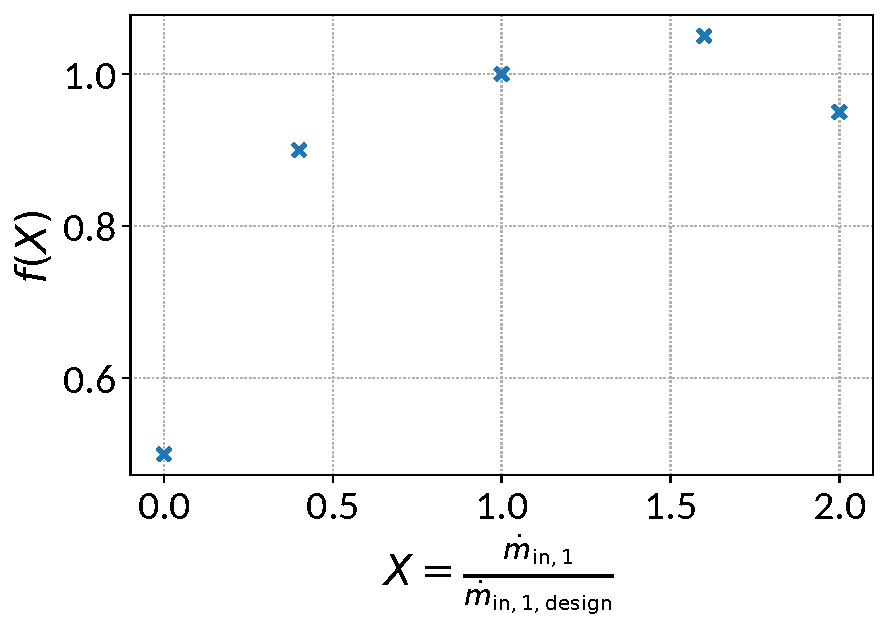
\includegraphics[width=\textwidth]{figures/Compressor_CharLine_eta_s_char_compressor.pdf}
\caption{Characteristics of compressor (eq. \ref{eq:Compressor_eta_s_char})}
\label{fig:CharLine_eta_s_char_compressor}
\end{center}\end{figure}

\end{minipage}
\begin{minipage}{0.5\textwidth}
\begin{figure}[H]\begin{center}
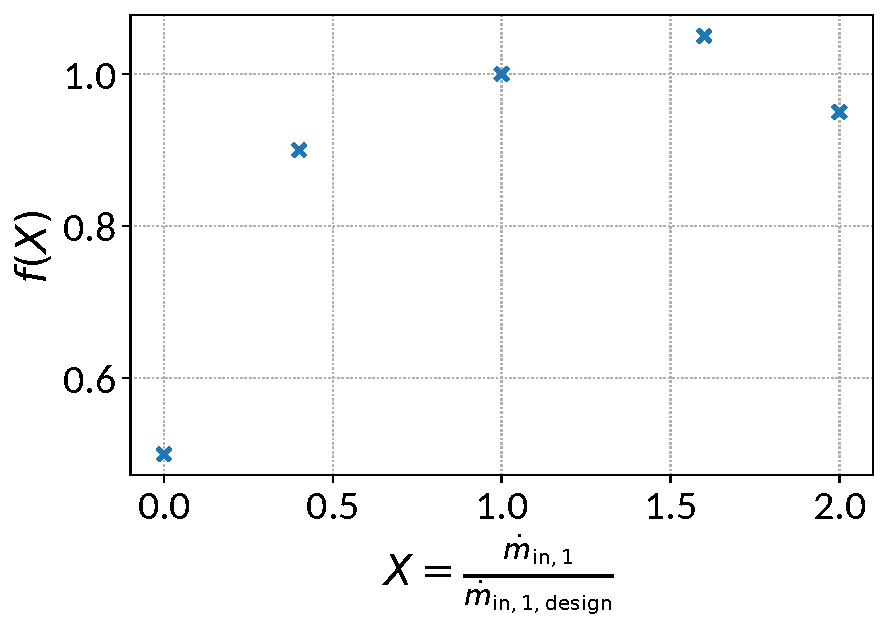
\includegraphics[width=\textwidth]{figures/Compressor_CharLine_eta_s_char_fuel_compressor.pdf}
\caption{Characteristics of fuel compressor (eq. \ref{eq:Compressor_eta_s_char})}
\label{fig:CharLine_eta_s_char_fuel compressor}
\end{center}\end{figure}

\end{minipage}


\subsection{Components of type CombustionChamber}

\subsubsection{Mandatory constraints}

\begin{equation}
\label{eq:CombustionChamber_mass_flow_constraints}
0=\dot{m}_\mathrm{in,1} + \dot{m}_\mathrm{in,2} - \dot{m}_\mathrm{out,1}
\end{equation}

\begin{equation}
\label{eq:CombustionChamber_reactor_pressure_constraints}
\begin{split}
0 = & p_\mathrm{in,1} - p_\mathrm{out,1}\\
0 = & p_\mathrm{in,1} - p_\mathrm{in,2}\\
\end{split}
\end{equation}

\begin{equation}
\label{eq:CombustionChamber_stoichiometry_constraints_general_eq}
\begin{split}
&\Delta \dot{m}_\mathrm{fluid} = \dot{m}_\mathrm{in,1} \cdot x_\mathrm{fluid,in,1} +\dot{m}_\mathrm{in,2} \cdot x_\mathrm{fluid,in,2}-\dot{m}_\mathrm{out,1} \cdot x_\mathrm{fluid,out,1}\\
&\dot{m}_\mathrm{fluid,m} = \frac{\dot{m}_\mathrm{in,1} \cdot x_\mathrm{fluid,in,1} +\dot{m}_\mathrm{in,2} \cdot x_\mathrm{fluid,in,2}}{M_\mathrm{fluid}}\\
&\dot{m}_\mathrm{H,m}=\dot{m}_\mathrm{CH4,m} \cdot 4\\
&\dot{m}_\mathrm{C,m}=\dot{m}_\mathrm{CH4,m} \cdot 1\\
&\dot{m}_\mathrm{O2,m,stoich}=\frac{\dot{m}_\mathrm{H,m}}{4} + \dot{m}_\mathrm{C,m}\\
\end{split}
\end{equation}
\begin{equation}
\label{eq:CombustionChamber_stoichiometry_constraints_Ar}
0 = \Delta \dot{m}_\mathrm{Ar}
\end{equation}
\begin{equation}
\label{eq:CombustionChamber_stoichiometry_constraints_CH4}
0=\Delta\dot{m}_\mathrm{CH4}-\dot{m}_\mathrm{CH4,m} \cdot M_\mathrm{CH4}
\end{equation}
\begin{equation}
\label{eq:CombustionChamber_stoichiometry_constraints_CO2}
0=\Delta \dot{m}_\mathrm{CO2} + \dot{m}_\mathrm{C,m} \cdot M_\mathrm{CO2} 
\end{equation}
\begin{equation}
\label{eq:CombustionChamber_stoichiometry_constraints_H2O}
0=\Delta \dot{m}_\mathrm{H2O} + \frac{\dot{m}_\mathrm{H,m}}{2} \cdot M_\mathrm{H2O} 
\end{equation}
\begin{equation}
\label{eq:CombustionChamber_stoichiometry_constraints_N2}
0 = \Delta \dot{m}_\mathrm{N2}
\end{equation}
\begin{equation}
\label{eq:CombustionChamber_stoichiometry_constraints_O2}
0=\Delta\dot{m}_\mathrm{O2}-\dot{m}_\mathrm{O2,m,stoich} \cdot M_\mathrm{O2}
\end{equation}

\begin{equation}
\label{eq:CombustionChamber_energy_balance_constraints}
\begin{split}
0 = & \sum_i \dot{m}_{\mathrm{in,}i} \cdot\left( h_{\mathrm{in,}i} - h_{\mathrm{in,}i\mathrm{,ref}} \right) -\dot{m}_\mathrm{out,1}\cdot\left( h_\mathrm{out,1} - h_\mathrm{out,1,ref}\right)\\
& + LHV_{fuel} \cdot \left(\sum_i \dot{m}_{\mathrm{in,}i} \cdot x_{fuel\mathrm{,in,}i} - \dot{m}_\mathrm{out,1} \cdot x_{fuel\mathrm{,out,1}} \right)\\
& \forall i \in \text{inlets}\\& T_\mathrm{ref}=\unit[298.15]{K}\;p_\mathrm{ref}=\unit[10^5]{Pa}\\
\end{split}
\end{equation}


\subsubsection{Specifications and results}

\begin{table}[H]
\centering
\caption{Parameters of components of type CombustionChamber}
\begin{tabular}{lrr}
\toprule
{} & lamb (\ref{eq:CombustionChamber_lamb}) &              ti \\
label      &                                        &                 \\
\midrule
combustion &                            \bftab 2.50 &  688,453,526.74 \\
\bottomrule
\end{tabular}
\end{table}
\subsubsection{Equations applied}

\begin{equation}
\label{eq:CombustionChamber_lamb}
\begin{split}
0 = \frac{\dot{m}_\mathrm{fuel,m}}{\dot{m}_\mathrm{O_2,m} \cdot \left(n_\mathrm{C,fuel} + 0.25 \cdot n_\mathrm{H,fuel}\right)} - \lambda \\
\dot{m}_\mathrm{fluid,m} = \frac{x_\mathrm{fluid} \cdot \dot{m}}{M_\mathrm{fluid}}\\
\end{split}
\end{equation}


\subsection{Components of type Turbine}

\subsubsection{Mandatory constraints}

\begin{equation}
\label{eq:Turbine_mass_flow_constraints}
0=\dot{m}_{\mathrm{in,}i}-\dot{m}_{\mathrm{out,}i}\; \forall i \in [1]
\end{equation}

\begin{equation}
\label{eq:Turbine_fluid_constraints}
0=x_{fl\mathrm{,in,}i}-x_{fl\mathrm{,out,}i}\;\forall fl \in\text{network fluids,}\; \forall i \in [1]
\end{equation}


\subsubsection{Specifications and results}

\begin{table}[H]
\centering
\caption{Parameters of components of type Turbine}
\begin{tabular}{lrrrr}
\toprule
{} &                P & eta\_s &    pr &  eta\_s\_char (\ref{eq:Turbine_eta_s_char}) \\
label                       &                  &        &       &                                             \\
\midrule
gas turbine                 &  -506,194,309.40 &   0.90 &  0.07 &                                        True \\
steam turbine high pressure &  -117,835,199.61 &   0.88 &  0.00 &                                        True \\
steam turbine low pressure  &   -21,384,531.22 &   0.88 &  0.16 &                                        True \\
\bottomrule
\end{tabular}
\end{table}
\subsubsection{Equations applied}

\begin{equation}
\label{eq:Turbine_eta_s_char}
0=-\left(h_\mathrm{out}-h_\mathrm{in}\right)+\eta_\mathrm{s,design}\cdot f \left(X\right)\cdot\left(h_\mathrm{out,s}-h_\mathrm{in}\right)
\end{equation}

\begin{minipage}{0.5\textwidth}
\begin{figure}[H]\begin{center}
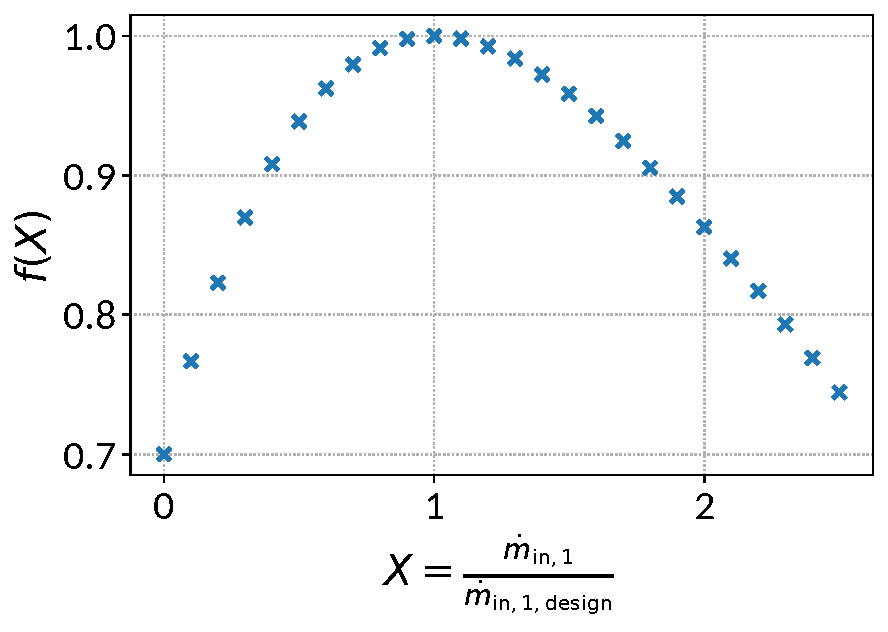
\includegraphics[width=\textwidth]{figures/Turbine_CharLine_eta_s_char_gas_turbine.pdf}
\caption{Characteristics of gas turbine (eq. \ref{eq:Turbine_eta_s_char})}
\label{fig:CharLine_eta_s_char_gas turbine}
\end{center}\end{figure}

\end{minipage}
\begin{minipage}{0.5\textwidth}
\begin{figure}[H]\begin{center}
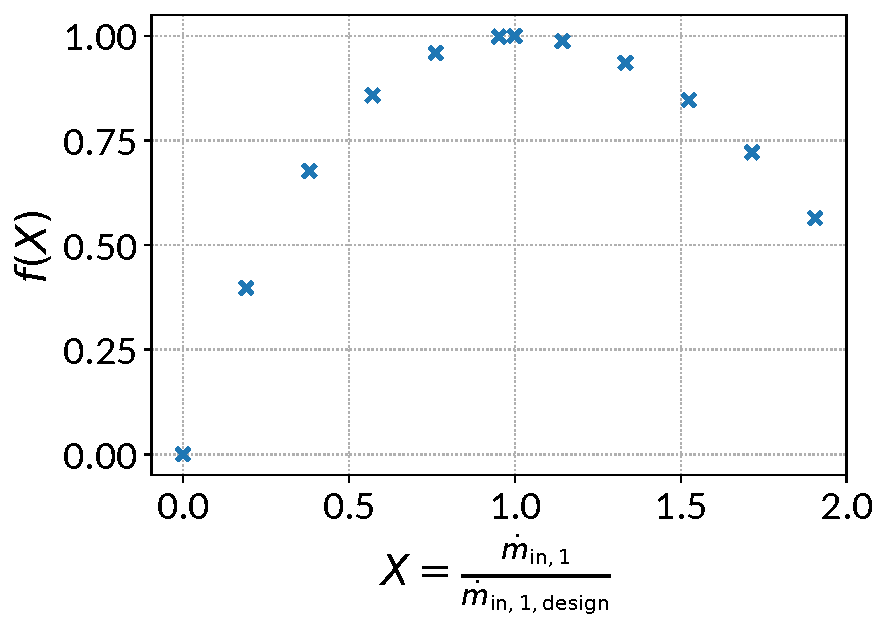
\includegraphics[width=\textwidth]{figures/Turbine_CharLine_eta_s_char_steam_turbine_high_pressure.pdf}
\caption{Characteristics of steam turbine high pressure (eq. \ref{eq:Turbine_eta_s_char})}
\label{fig:CharLine_eta_s_char_steam turbine high pressure}
\end{center}\end{figure}

\end{minipage}

\begin{minipage}{0.5\textwidth}
\begin{figure}[H]\begin{center}
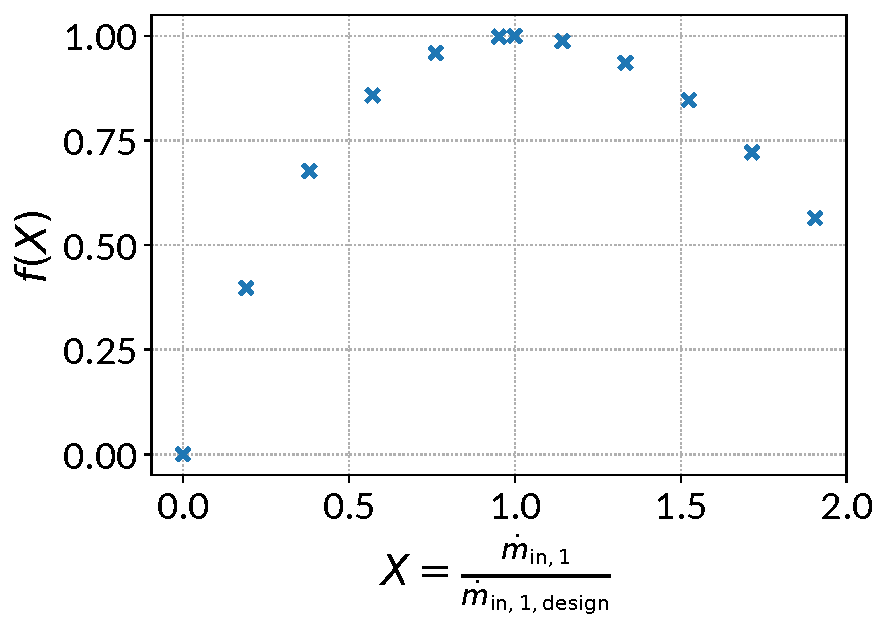
\includegraphics[width=\textwidth]{figures/Turbine_CharLine_eta_s_char_steam_turbine_low_pressure.pdf}
\caption{Characteristics of steam turbine low pressure (eq. \ref{eq:Turbine_eta_s_char})}
\label{fig:CharLine_eta_s_char_steam turbine low pressure}
\end{center}\end{figure}

\end{minipage}

\subsection{Components of type HeatExchanger}

\subsubsection{Mandatory constraints}

\begin{equation}
\label{eq:HeatExchanger_mass_flow_constraints}
0=\dot{m}_{\mathrm{in,}i}-\dot{m}_{\mathrm{out,}i}\; \forall i \in [1, 2]
\end{equation}

\begin{equation}
\label{eq:HeatExchanger_fluid_constraints}
0=x_{fl\mathrm{,in,}i}-x_{fl\mathrm{,out,}i}\;\forall fl \in\text{network fluids,}\; \forall i \in [1, 2]
\end{equation}

\begin{equation}
\label{eq:HeatExchanger_energy_balance_constraints}
0 = \dot{m}_\mathrm{in,1} \cdot \left(h_\mathrm{out,1} - h_\mathrm{in,1} \right) +\dot{m}_\mathrm{in,2} \cdot \left(h_\mathrm{out,2} - h_\mathrm{in,2} \right)
\end{equation}


\subsubsection{Specifications and results}

\begin{table}[H]
\centering
\caption{Parameters of components of type HeatExchanger}
\begin{tabular}{lrrrrrrrrrr}
\toprule
{} &                Q &            kA & td\_log &  ttd\_u &  ttd\_l &   pr1 &   pr2 & zeta1 (\ref{eq:HeatExchanger_zeta1}) & zeta2 (\ref{eq:HeatExchanger_zeta2}) &  kA\_char (\ref{eq:HeatExchanger_kA_char}) \\
label       &                  &               &         &         &         &       &       &                                      &                                      &                                            \\
\midrule
superheater &   -98,614,527.98 &    949,815.67 &  103.82 &   50.00 &  186.90 &  0.99 &  0.98 &                          \bftab 0.00 &                      \bftab 1,492.03 &                                       True \\
evaporator  &  -115,208,431.13 &  1,542,695.55 &   74.68 &  186.90 &   20.00 &  0.99 &  1.00 &                          \bftab 0.00 &                                 0.00 &                                       True \\
economizer  &  -138,983,332.78 &  2,677,700.13 &   51.90 &   21.39 &  102.94 &  0.99 &  1.00 &                          \bftab 0.00 &                          \bftab 0.00 &                                       True \\
\bottomrule
\end{tabular}
\end{table}
\subsubsection{Equations applied}

\begin{equation}
\label{eq:HeatExchanger_zeta1}
0 = \begin{cases}
p_\mathrm{in,1}- p_\mathrm{out,1} & |\dot{m}_\mathrm{in,1}| < \unitfrac[0.0001]{kg}{s} \\
\frac{\zeta}{D^4}-\frac{(p_\mathrm{in,1}-p_\mathrm{out,1})\cdot\pi^2}{8\cdot\dot{m}_\mathrm{in,1}\cdot|\dot{m}_\mathrm{in,1}|\cdot\frac{v_\mathrm{in,1} + v_\mathrm{out,1}}{2}}& |\dot{m}_\mathrm{in,1}| \geq \unitfrac[0.0001]{kg}{s}
\end{cases}
\end{equation}

\begin{equation}
\label{eq:HeatExchanger_zeta2}
0 = \begin{cases}
p_\mathrm{in,2}- p_\mathrm{out,2} & |\dot{m}_\mathrm{in,2}| < \unitfrac[0.0001]{kg}{s} \\
\frac{\zeta}{D^4}-\frac{(p_\mathrm{in,2}-p_\mathrm{out,2})\cdot\pi^2}{8\cdot\dot{m}_\mathrm{in,2}\cdot|\dot{m}_\mathrm{in,2}|\cdot\frac{v_\mathrm{in,2} + v_\mathrm{out,2}}{2}}& |\dot{m}_\mathrm{in,2}| \geq \unitfrac[0.0001]{kg}{s}
\end{cases}
\end{equation}

\begin{equation}
\label{eq:HeatExchanger_kA_char}
\begin{split}
0 = & \dot{m}_\mathrm{in,1} \cdot \left( h_\mathrm{out,1} - h_\mathrm{in,1}\right)\\
&+kA_\mathrm{design} \cdot f_\mathrm{kA} \cdot \frac{T_\mathrm{out,1} - T_\mathrm{in,2} - T_\mathrm{in,1} + T_\mathrm{out,2}}{\ln{\frac{T_\mathrm{out,1} - T_\mathrm{in,2}}{T_\mathrm{in,1} - T_\mathrm{out,2}}}}\\
f_\mathrm{kA}=&\frac{2}{\frac{1}{f\left(X_1\right)}+\frac{1}{f\left(X_2\right)}}\\
\end{split}
\end{equation}

\begin{minipage}{0.5\textwidth}
\begin{figure}[H]\begin{center}
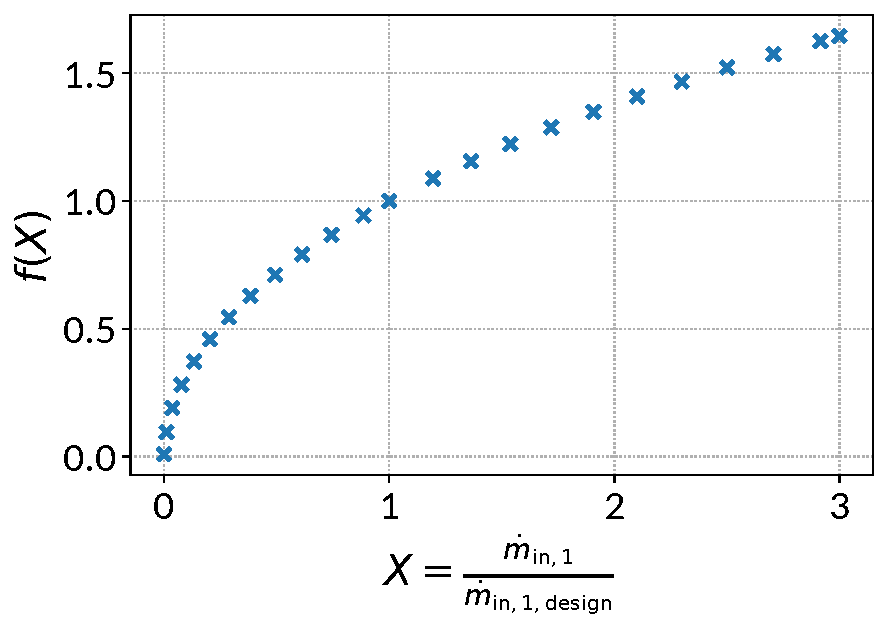
\includegraphics[width=\textwidth]{figures/HeatExchanger_CharLine_kA_char1_superheater.pdf}
\caption{Characteristics of superheater (eq. \ref{eq:HeatExchanger_kA_char})}
\label{fig:CharLine_kA_char1_superheater}
\end{center}\end{figure}

\end{minipage}
\begin{minipage}{0.5\textwidth}
\begin{figure}[H]\begin{center}
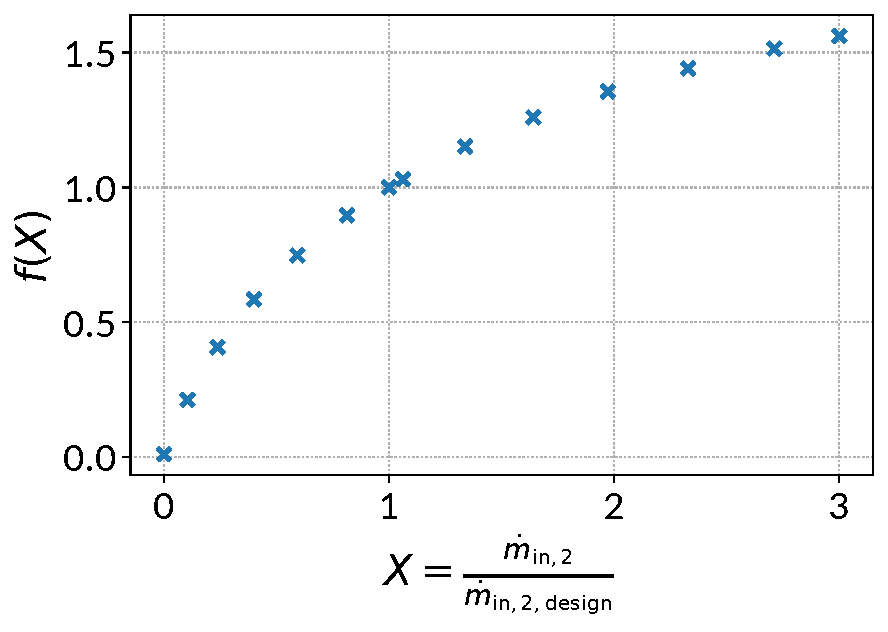
\includegraphics[width=\textwidth]{figures/HeatExchanger_CharLine_kA_char2_superheater.pdf}
\caption{Characteristics of superheater (eq. \ref{eq:HeatExchanger_kA_char})}
\label{fig:CharLine_kA_char2_superheater}
\end{center}\end{figure}

\end{minipage}

\begin{minipage}{0.5\textwidth}
\begin{figure}[H]\begin{center}
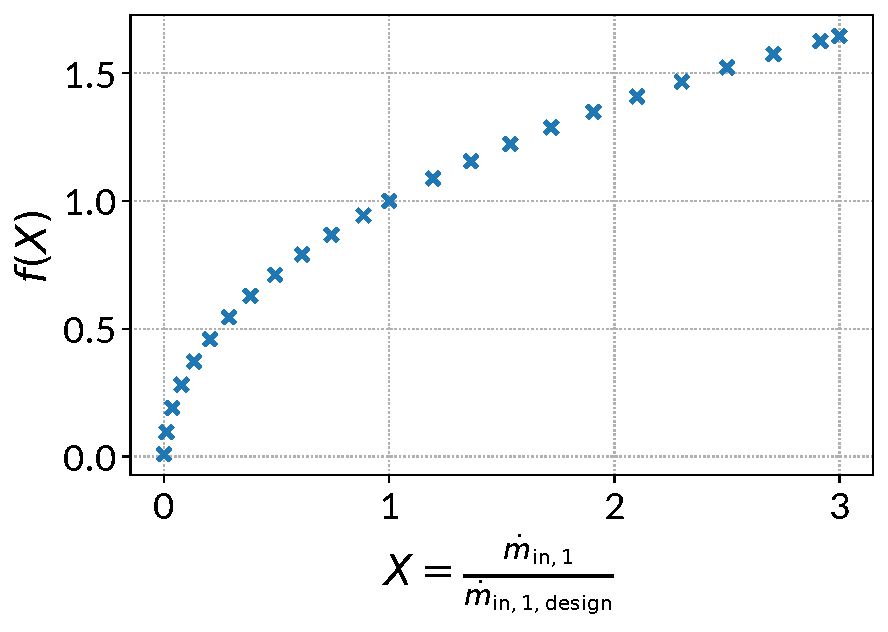
\includegraphics[width=\textwidth]{figures/HeatExchanger_CharLine_kA_char1_evaporator.pdf}
\caption{Characteristics of evaporator (eq. \ref{eq:HeatExchanger_kA_char})}
\label{fig:CharLine_kA_char1_evaporator}
\end{center}\end{figure}

\end{minipage}
\begin{minipage}{0.5\textwidth}
\begin{figure}[H]\begin{center}
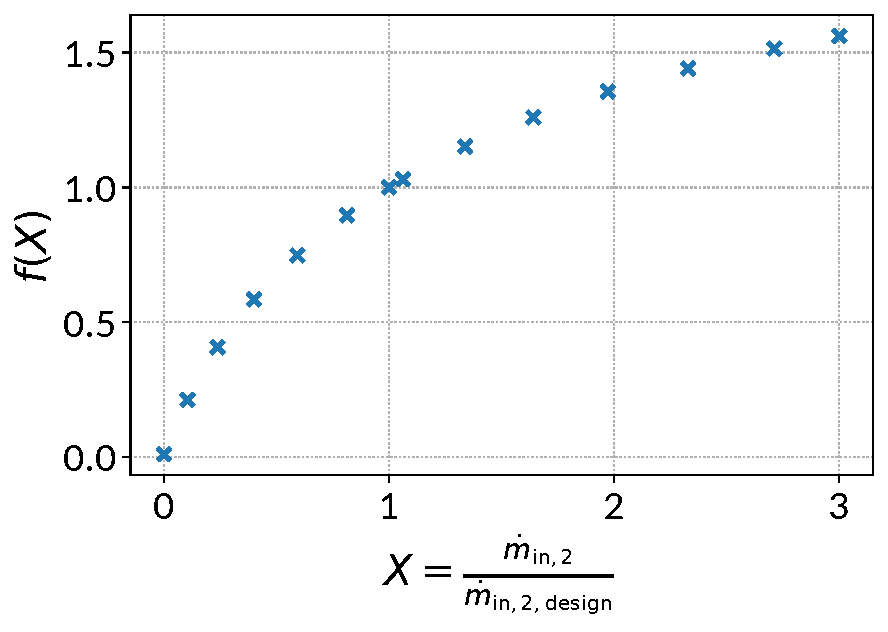
\includegraphics[width=\textwidth]{figures/HeatExchanger_CharLine_kA_char2_evaporator.pdf}
\caption{Characteristics of evaporator (eq. \ref{eq:HeatExchanger_kA_char})}
\label{fig:CharLine_kA_char2_evaporator}
\end{center}\end{figure}

\end{minipage}

\begin{minipage}{0.5\textwidth}
\begin{figure}[H]\begin{center}
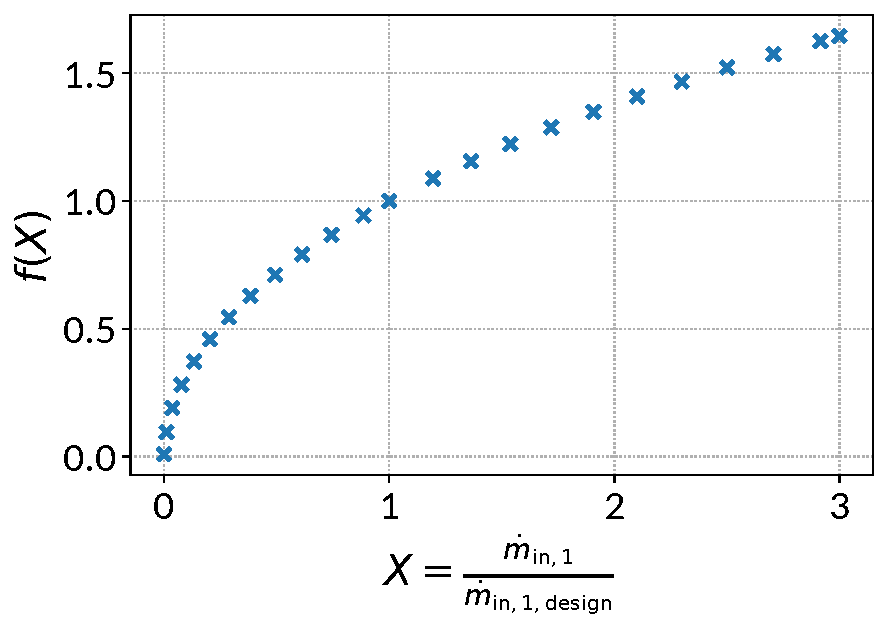
\includegraphics[width=\textwidth]{figures/HeatExchanger_CharLine_kA_char1_economizer.pdf}
\caption{Characteristics of economizer (eq. \ref{eq:HeatExchanger_kA_char})}
\label{fig:CharLine_kA_char1_economizer}
\end{center}\end{figure}

\end{minipage}
\begin{minipage}{0.5\textwidth}
\begin{figure}[H]\begin{center}
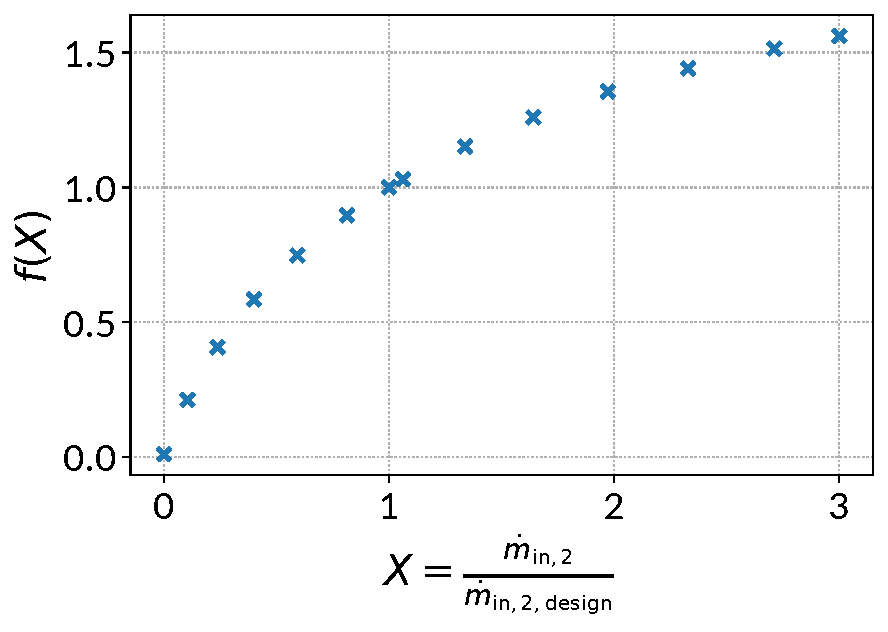
\includegraphics[width=\textwidth]{figures/HeatExchanger_CharLine_kA_char2_economizer.pdf}
\caption{Characteristics of economizer (eq. \ref{eq:HeatExchanger_kA_char})}
\label{fig:CharLine_kA_char2_economizer}
\end{center}\end{figure}

\end{minipage}


\subsection{Components of type Drum}

\subsubsection{Mandatory constraints}

\begin{equation}
\label{eq:Drum_mass_flow_constraints}
0 =\sum\dot{m}_{\mathrm{in},i}-\sum\dot{m}_{\mathrm{out},j}\;\forall i \in \text{inlets}, \forall j \in \text{outlets}
\end{equation}

\begin{equation}
\label{eq:Drum_fluid_constraints}
0 = x_{fl\mathrm{,in,1}} - x_{fl\mathrm{,out,}j}\; \forall fl \in \text{network fluids,} \; \forall j \in\text{outlets}
\end{equation}

\begin{equation}
\label{eq:Drum_energy_balance_constraints}
0=\sum_i\left(\dot{m}_{\mathrm{in,}i}\cdot h_{\mathrm{in,}i}\right) - \sum_j \left(\dot{m}_{\mathrm{out,}j} \cdot h_{\mathrm{out,}j} \right) \; \forall i \in \text{inlets} \;\forall j \in \text{outlets}
\end{equation}

\begin{equation}
\label{eq:Drum_pressure_constraints}
\begin{split}
0 = p_\mathrm{in,1} - p_{\mathrm{in,}i} & \; \forall i \in \text{inlets} \setminus \left\lbrace 1\right\rbrace\\
0 = p_\mathrm{in,1} - p_{\mathrm{out,}j} & \; \forall j \in \text{outlets}\\
\end{split}
\end{equation}

\begin{equation}
\label{eq:Drum_outlet_constraints}
\begin{split}
0 =&h_\mathrm{out,1} -h\left(p_\mathrm{out,1}, x=0\right)\\0 =&h_\mathrm{out,2} -h\left(p_\mathrm{out,2}, x=1\right)\\\end{split}
\end{equation}


\subsection{Components of type Splitter}

\subsubsection{Mandatory constraints}

\begin{equation}
\label{eq:Splitter_mass_flow_constraints}
0 =\sum\dot{m}_{\mathrm{in},i}-\sum\dot{m}_{\mathrm{out},j}\;\forall i \in \text{inlets}, \forall j \in \text{outlets}
\end{equation}

\begin{equation}
\label{eq:Splitter_fluid_constraints}
0 = x_{fl\mathrm{,in}} - x_{fl\mathrm{,out,}j}\; \forall fl \in \text{network fluids,} \; \forall j \in\text{outlets}
\end{equation}

\begin{equation}
\label{eq:Splitter_energy_balance_constraints}
0=h_{in}-h_{\mathrm{out,}j}\;\forall j \in\text{outlets}
\end{equation}

\begin{equation}
\label{eq:Splitter_pressure_constraints}
\begin{split}
0 = p_\mathrm{in,1} - p_{\mathrm{in,}i} & \; \forall i \in \text{inlets} \setminus \left\lbrace 1\right\rbrace\\
0 = p_\mathrm{in,1} - p_{\mathrm{out,}j} & \; \forall j \in \text{outlets}\\
\end{split}
\end{equation}


\subsection{Components of type Condenser}

\subsubsection{Mandatory constraints}

\begin{equation}
\label{eq:Condenser_mass_flow_constraints}
0=\dot{m}_{\mathrm{in,}i}-\dot{m}_{\mathrm{out,}i}\; \forall i \in [1, 2]
\end{equation}

\begin{equation}
\label{eq:Condenser_fluid_constraints}
0=x_{fl\mathrm{,in,}i}-x_{fl\mathrm{,out,}i}\;\forall fl \in\text{network fluids,}\; \forall i \in [1, 2]
\end{equation}

\begin{equation}
\label{eq:Condenser_energy_balance_constraints}
0 = \dot{m}_\mathrm{in,1} \cdot \left(h_\mathrm{out,1} - h_\mathrm{in,1} \right) +\dot{m}_\mathrm{in,2} \cdot \left(h_\mathrm{out,2} - h_\mathrm{in,2} \right)
\end{equation}


\subsubsection{Specifications and results}

\begin{table}[H]
\centering
\caption{Parameters of components of type Condenser}
\begin{tabular}{lrrrrrrrrrr}
\toprule
{} &                Q &             kA & td\_log &  ttd\_u & ttd\_l & pr1 (\ref{eq:Condenser_pr1}) &   pr2 &  zeta1 & zeta2 (\ref{eq:Condenser_zeta2}) &  kA\_char (\ref{eq:Condenser_kA_char}) \\
label                      &                  &                &         &         &        &                              &       &        &                                  &                                        \\
\midrule
district heating condenser &   -10,000,000.00 &              - &       - &  -16.67 &  23.09 &                  \bftab 0.99 &  1.00 &  10.12 &                     \bftab 18.94 &                                   True \\
condenser                  &  -205,865,521.11 &  19,132,458.10 &   10.76 &    5.00 &  19.82 &                  \bftab 0.99 &  0.98 &   0.00 &                      \bftab 1.14 &                                   True \\
\bottomrule
\end{tabular}
\end{table}
\subsubsection{Equations applied}

\begin{equation}
\label{eq:Condenser_pr1}
0=p_\mathrm{in,1}\cdot pr1 - p_\mathrm{out,1}
\end{equation}

\begin{equation}
\label{eq:Condenser_zeta2}
0 = \begin{cases}
p_\mathrm{in,2}- p_\mathrm{out,2} & |\dot{m}_\mathrm{in,2}| < \unitfrac[0.0001]{kg}{s} \\
\frac{\zeta}{D^4}-\frac{(p_\mathrm{in,2}-p_\mathrm{out,2})\cdot\pi^2}{8\cdot\dot{m}_\mathrm{in,2}\cdot|\dot{m}_\mathrm{in,2}|\cdot\frac{v_\mathrm{in,2} + v_\mathrm{out,2}}{2}}& |\dot{m}_\mathrm{in,2}| \geq \unitfrac[0.0001]{kg}{s}
\end{cases}
\end{equation}

\begin{equation}
\label{eq:Condenser_kA_char}
\begin{split}
0 = & \dot{m}_\mathrm{in,1} \cdot \left( h_\mathrm{out,1} - h_\mathrm{in,1}\right)\\
&+kA_\mathrm{design} \cdot f_\mathrm{kA} \cdot \frac{T_\mathrm{out,1} - T_\mathrm{in,2} - T_\mathrm{sat}\left( p_\mathrm{in,1}\right) +T_\mathrm{out,2}}{\ln{\frac{T_\mathrm{out,1}-T_\mathrm{in,2}}{T_\mathrm{sat}\left( p_\mathrm{in,1}\right)- T_\mathrm{out,2}}}}\\
f_\mathrm{kA}=&\frac{2}{\frac{1}{f\left(X_1\right)}+\frac{1}{f\left(X_2\right)}}\\
\end{split}
\end{equation}

\begin{minipage}{0.5\textwidth}
\begin{figure}[H]\begin{center}
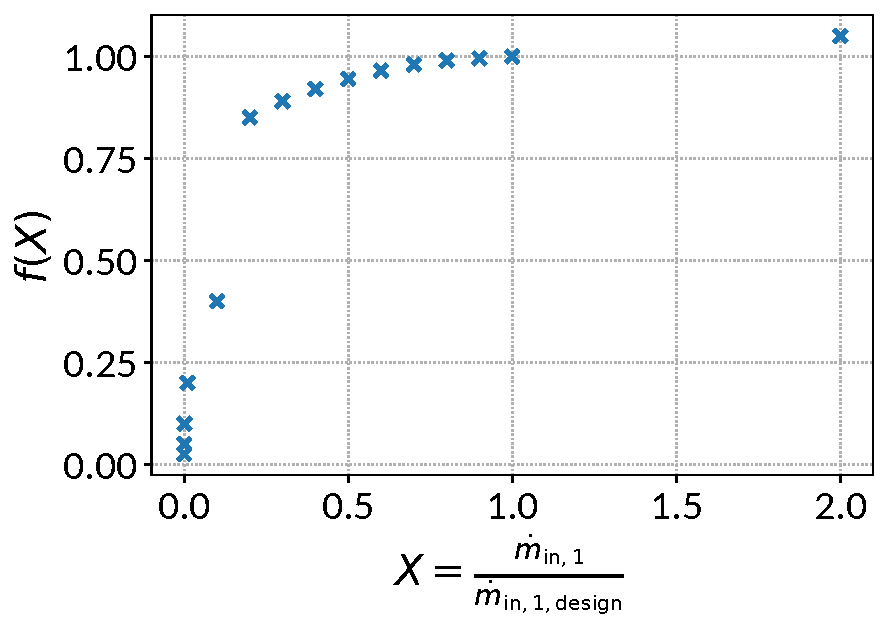
\includegraphics[width=\textwidth]{figures/Condenser_CharLine_kA_char1_district_heating_condenser.pdf}
\caption{Characteristics of district heating condenser (eq. \ref{eq:Condenser_kA_char})}
\label{fig:CharLine_kA_char1_district heating condenser}
\end{center}\end{figure}

\end{minipage}
\begin{minipage}{0.5\textwidth}
\begin{figure}[H]\begin{center}
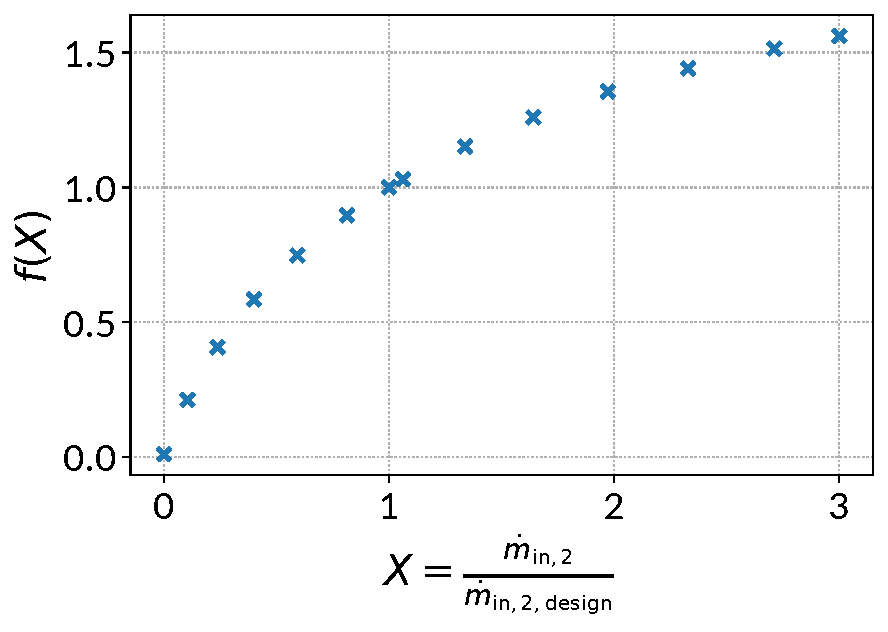
\includegraphics[width=\textwidth]{figures/Condenser_CharLine_kA_char2_district_heating_condenser.pdf}
\caption{Characteristics of district heating condenser (eq. \ref{eq:Condenser_kA_char})}
\label{fig:CharLine_kA_char2_district heating condenser}
\end{center}\end{figure}

\end{minipage}

\begin{minipage}{0.5\textwidth}
\begin{figure}[H]\begin{center}
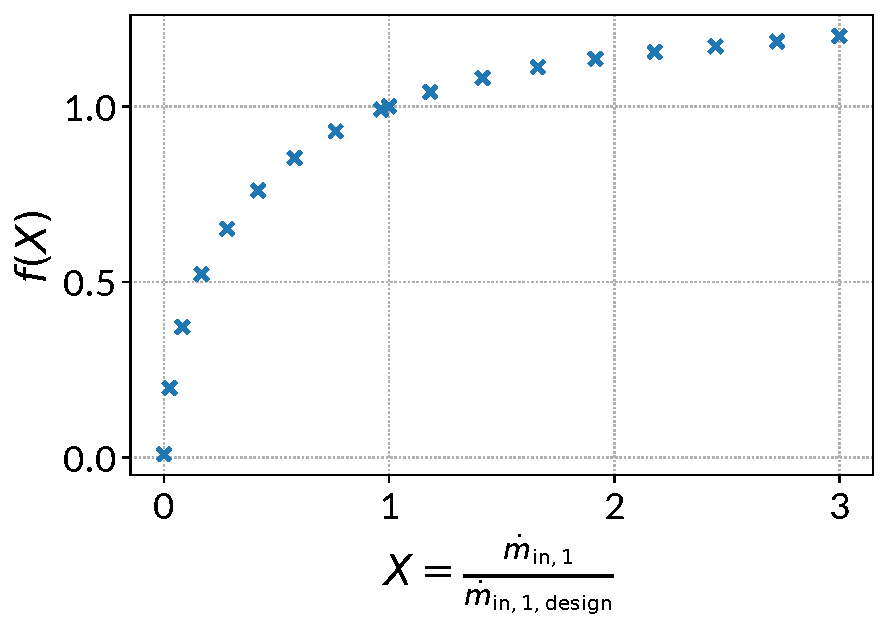
\includegraphics[width=\textwidth]{figures/Condenser_CharLine_kA_char1_condenser.pdf}
\caption{Characteristics of condenser (eq. \ref{eq:Condenser_kA_char})}
\label{fig:CharLine_kA_char1_condenser}
\end{center}\end{figure}

\end{minipage}
\begin{minipage}{0.5\textwidth}
\begin{figure}[H]\begin{center}
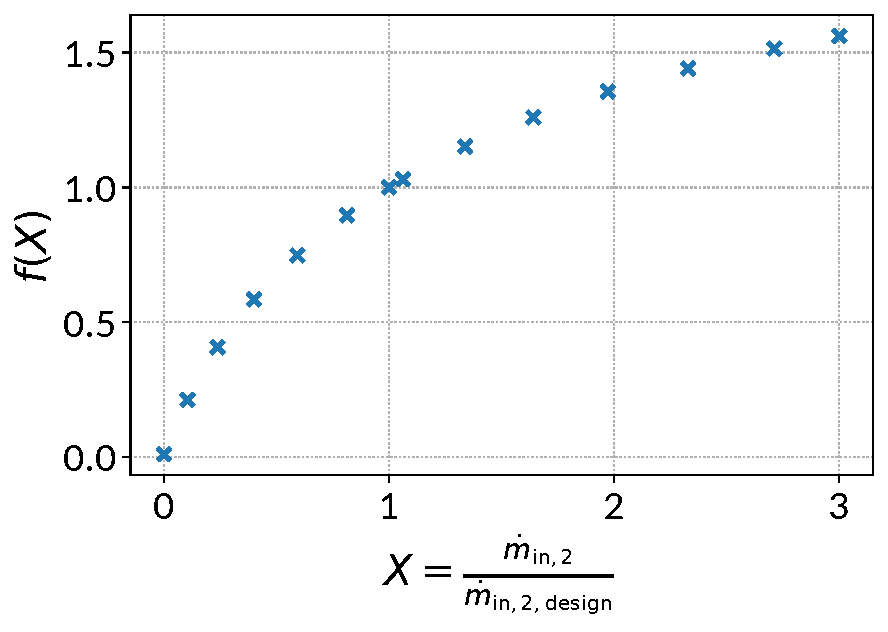
\includegraphics[width=\textwidth]{figures/Condenser_CharLine_kA_char2_condenser.pdf}
\caption{Characteristics of condenser (eq. \ref{eq:Condenser_kA_char})}
\label{fig:CharLine_kA_char2_condenser}
\end{center}\end{figure}

\end{minipage}


\subsection{Components of type Pump}

\subsubsection{Mandatory constraints}

\begin{equation}
\label{eq:Pump_mass_flow_constraints}
0=\dot{m}_{\mathrm{in,}i}-\dot{m}_{\mathrm{out,}i}\; \forall i \in [1]
\end{equation}

\begin{equation}
\label{eq:Pump_fluid_constraints}
0=x_{fl\mathrm{,in,}i}-x_{fl\mathrm{,out,}i}\;\forall fl \in\text{network fluids,}\; \forall i \in [1]
\end{equation}


\subsubsection{Specifications and results}

\begin{table}[H]
\centering
\caption{Parameters of components of type Pump}
\begin{tabular}{lrrrr}
\toprule
{} &             P & eta\_s &        pr &  eta\_s\_char (\ref{eq:Pump_eta_s_char}) \\
label             &               &        &           &                                          \\
\midrule
feed water pump 1 &    652,354.48 &   0.10 &    372.45 &                                     True \\
feed water pump 2 &  1,626,605.57 &   0.80 &  2,380.40 &                                     True \\
\bottomrule
\end{tabular}
\end{table}
\subsubsection{Equations applied}

\begin{equation}
\label{eq:Pump_eta_s_char}
0=\left(h_\mathrm{out}-h_\mathrm{in}\right)\cdot\eta_\mathrm{s,design}\cdot f\left( X \right)-\left( h_{out,s} - h_{in} \right)
\end{equation}

\begin{minipage}{0.5\textwidth}
\begin{figure}[H]\begin{center}
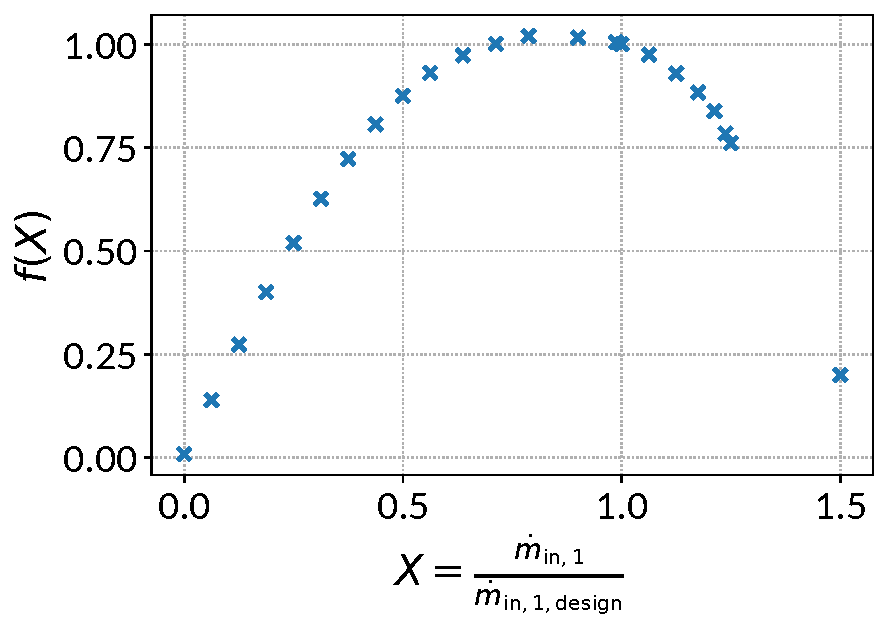
\includegraphics[width=\textwidth]{figures/Pump_CharLine_eta_s_char_feed_water_pump_1.pdf}
\caption{Characteristics of feed water pump 1 (eq. \ref{eq:Pump_eta_s_char})}
\label{fig:CharLine_eta_s_char_feed water pump 1}
\end{center}\end{figure}

\end{minipage}
\begin{minipage}{0.5\textwidth}
\begin{figure}[H]\begin{center}
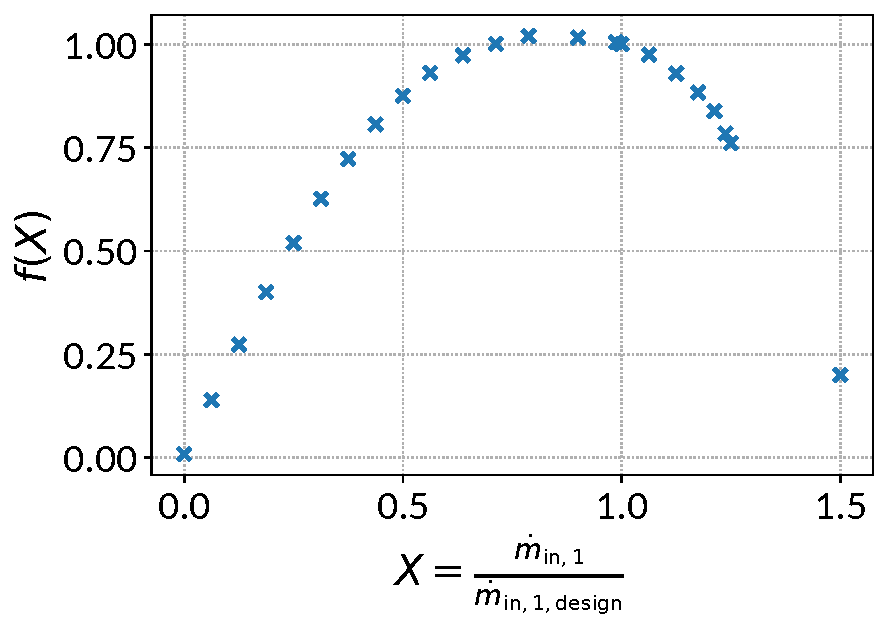
\includegraphics[width=\textwidth]{figures/Pump_CharLine_eta_s_char_feed_water_pump_2.pdf}
\caption{Characteristics of feed water pump 2 (eq. \ref{eq:Pump_eta_s_char})}
\label{fig:CharLine_eta_s_char_feed water pump 2}
\end{center}\end{figure}

\end{minipage}


\subsection{Components of type Merge}

\subsubsection{Mandatory constraints}

\begin{equation}
\label{eq:Merge_mass_flow_constraints}
0 =\sum\dot{m}_{\mathrm{in},i}-\sum\dot{m}_{\mathrm{out},j}\;\forall i \in \text{inlets}, \forall j \in \text{outlets}
\end{equation}

\begin{equation}
\label{eq:Merge_fluid_constraints}
0=\sum_i \dot{m}_{\mathrm{in,}i} \cdot x_{fl\mathrm{,in,}i}- \dot {m}_\mathrm{out} \cdot x_{fl\mathrm{,out}}\; \forall fl \in \text{network fluids,} \; \forall i \in\text{inlets}
\end{equation}

\begin{equation}
\label{eq:Merge_energy_balance_constraints}
0=\sum_i\left(\dot{m}_{\mathrm{in,}i}\cdot h_{\mathrm{in,}i}\right) - \dot{m}_\mathrm{out} \cdot h_\mathrm{out} \; \forall i \in \text{inlets}
\end{equation}

\begin{equation}
\label{eq:Merge_pressure_constraints}
\begin{split}
0 = p_\mathrm{in,1} - p_{\mathrm{in,}i} & \; \forall i \in \text{inlets} \setminus \left\lbrace 1\right\rbrace\\
0 = p_\mathrm{in,1} - p_{\mathrm{out,}j} & \; \forall j \in \text{outlets}\\
\end{split}
\end{equation}


\subsection{Components of type Valve}

\subsubsection{Mandatory constraints}

\begin{equation}
\label{eq:Valve_mass_flow_constraints}
0=\dot{m}_{\mathrm{in,}i}-\dot{m}_{\mathrm{out,}i}\; \forall i \in [1]
\end{equation}

\begin{equation}
\label{eq:Valve_fluid_constraints}
0=x_{fl\mathrm{,in,}i}-x_{fl\mathrm{,out,}i}\;\forall fl \in\text{network fluids,}\; \forall i \in [1]
\end{equation}

\begin{equation}
\label{eq:Valve_enthalpy_equality_constraints}
0=h_{\mathrm{in,}i}-h_{\mathrm{out,}i}\; \forall i \in [1]
\end{equation}


\subsubsection{Specifications and results}

\begin{table}[H]
\centering
\caption{Parameters of components of type Valve}
\begin{tabular}{lrr}
\toprule
{} &    pr &   zeta \\
label    &       &        \\
\midrule
mp valve &  1.00 &  -0.00 \\
\bottomrule
\end{tabular}
\end{table}
\section{Busses in offdesign mode}

\subsection{Bus ``power output''}

This bus is used for postprocessing only.

\begin{table}[H]
\centering
\caption{Results overview for bus power output}
\begin{tabular}{lrrrrrr}
\toprule
{} &                                                   $\dot{E}_\mathrm{comp}$ & $\dot{E}_\mathrm{comp,result}$ &                $\dot{E}_\mathrm{bus}$ & $\dot{E}_\mathrm{bus,result}$ &                                                               $\eta$ & $\eta_\mathrm{result}$ \\
label                       &                                                                           &                                &                                       &                               &                                                                      &                        \\
\midrule
gas turbine                 &  $\dot{m}_\mathrm{in} \cdot \left(h_\mathrm{out} - h_\mathrm{in} \right)$ &                -506,194,309.40 &    $\dot{E}_\mathrm{comp} \cdot \eta$ &               -498,095,200.45 &      $f\left(X\right)$ (\ref{fig:Bus_CharLine_gas turbineoffdesign}) &                   0.98 \\
compressor                  &  $\dot{m}_\mathrm{in} \cdot \left(h_\mathrm{out} - h_\mathrm{in} \right)$ &                 239,522,262.15 &    $\dot{E}_\mathrm{comp} \cdot \eta$ &                239,522,262.15 &                                                                    - &                   1.00 \\
fuel compressor             &  $\dot{m}_\mathrm{in} \cdot \left(h_\mathrm{out} - h_\mathrm{in} \right)$ &                   9,173,521.53 &  $\frac{\dot{E}_\mathrm{comp}}{\eta}$ &                  9,457,238.69 &  $f\left(X\right)$ (\ref{fig:Bus_CharLine_fuel compressoroffdesign}) &                   0.97 \\
steam turbine high pressure &  $\dot{m}_\mathrm{in} \cdot \left(h_\mathrm{out} - h_\mathrm{in} \right)$ &                -117,835,199.61 &    $\dot{E}_\mathrm{comp} \cdot \eta$ &               -115,949,836.42 &      $f\left(X\right)$ (\ref{fig:Bus_CharLine_gas turbineoffdesign}) &                   0.98 \\
feed water pump 1           &  $\dot{m}_\mathrm{in} \cdot \left(h_\mathrm{out} - h_\mathrm{in} \right)$ &                     652,354.48 &  $\frac{\dot{E}_\mathrm{comp}}{\eta}$ &                    709,877.98 &  $f\left(X\right)$ (\ref{fig:Bus_CharLine_fuel compressoroffdesign}) &                   0.92 \\
steam turbine low pressure  &  $\dot{m}_\mathrm{in} \cdot \left(h_\mathrm{out} - h_\mathrm{in} \right)$ &                 -21,384,531.22 &    $\dot{E}_\mathrm{comp} \cdot \eta$ &                -21,042,378.72 &      $f\left(X\right)$ (\ref{fig:Bus_CharLine_gas turbineoffdesign}) &                   0.98 \\
feed water pump 2           &  $\dot{m}_\mathrm{in} \cdot \left(h_\mathrm{out} - h_\mathrm{in} \right)$ &                   1,626,605.57 &  $\frac{\dot{E}_\mathrm{comp}}{\eta}$ &                  1,676,912.96 &  $f\left(X\right)$ (\ref{fig:Bus_CharLine_fuel compressoroffdesign}) &                   0.97 \\
total                       &                                                                         - &                -394,439,296.51 &                                     - &               -383,721,123.81 &                                                                    - &                      - \\
\bottomrule
\end{tabular}
\end{table}


\begin{minipage}{0.5\textwidth}
\begin{figure}[H]\begin{center}
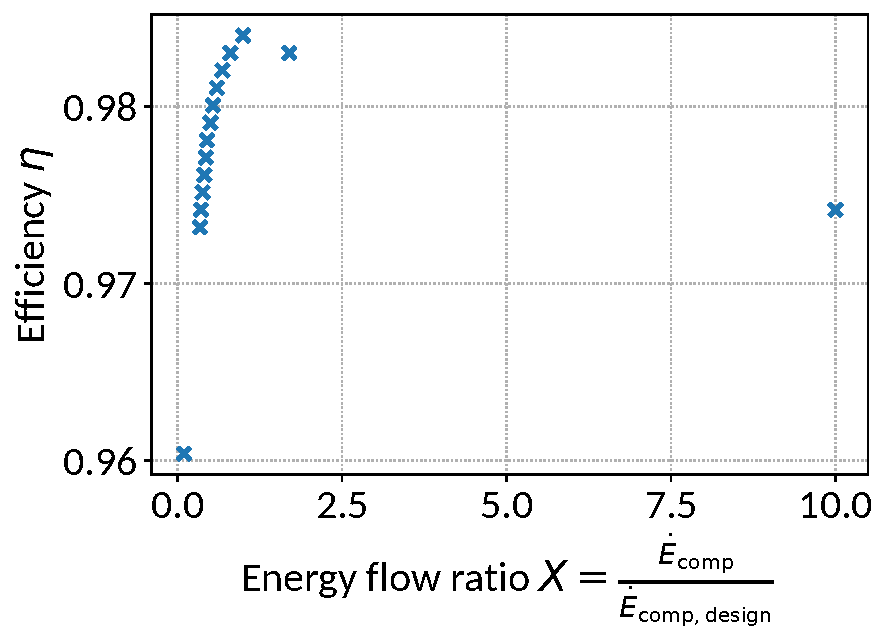
\includegraphics[width=\textwidth]{figures/Bus_CharLine_gas_turbineoffdesign.pdf}
\caption{Bus efficiency characteristic}
\label{fig:Bus_CharLine_gas turbineoffdesign}
\end{center}\end{figure}

\end{minipage}
\begin{minipage}{0.5\textwidth}
\begin{figure}[H]\begin{center}
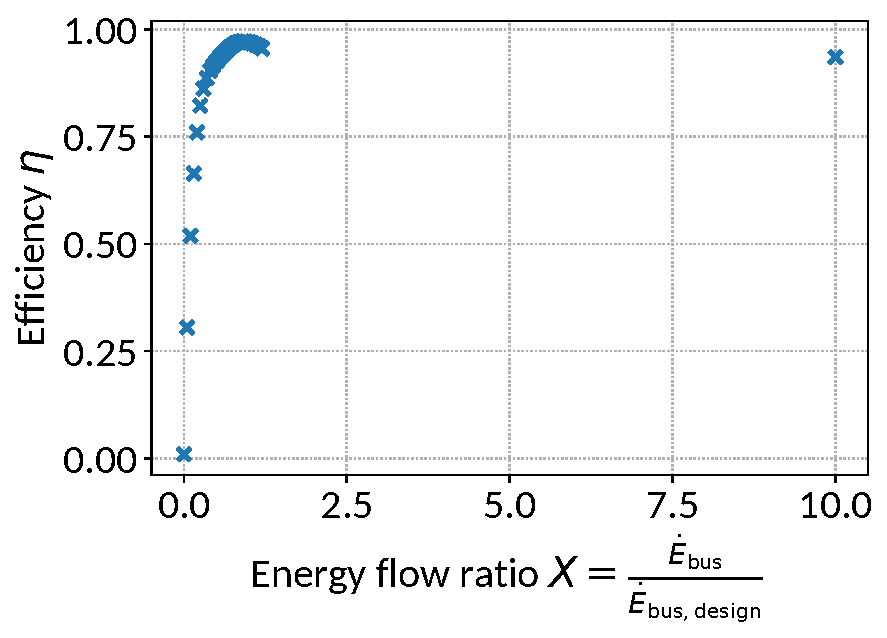
\includegraphics[width=\textwidth]{figures/Bus_CharLine_fuel_compressoroffdesign.pdf}
\caption{Bus efficiency characteristic}
\label{fig:Bus_CharLine_fuel compressoroffdesign}
\end{center}\end{figure}

\end{minipage}


\subsection{Bus ``gas turbine power output''}

Specified total value of energy flow: $\dot{E}_\mathrm{bus} = \unit[-266,672,047.25]{W}$

\begin{equation}
\label{eq:Bus_energy_flow_sum}
0=\dot{E}_\mathrm{bus} -\sum_i \dot{E}_{\mathrm{bus,}i}
\end{equation}

\begin{table}[H]
\centering
\caption{Results overview for bus gas turbine power output}
\begin{tabular}{lrrrrr}
\toprule
{} &                                                   $\dot{E}_\mathrm{comp}$ & $\dot{E}_\mathrm{comp,result}$ &              $\dot{E}_\mathrm{bus}$ & $\dot{E}_\mathrm{bus,result}$ & $\eta_\mathrm{result}$ \\
label       &                                                                           &                                &                                     &                               &                        \\
\midrule
gas turbine &  $\dot{m}_\mathrm{in} \cdot \left(h_\mathrm{out} - h_\mathrm{in} \right)$ &                -506,194,309.40 &  $\dot{E}_\mathrm{comp} \cdot \eta$ &               -506,194,309.40 &                   1.00 \\
compressor  &  $\dot{m}_\mathrm{in} \cdot \left(h_\mathrm{out} - h_\mathrm{in} \right)$ &                 239,522,262.15 &  $\dot{E}_\mathrm{comp} \cdot \eta$ &                239,522,262.15 &                   1.00 \\
total       &                                                                         - &                -266,672,047.25 &                                   - &         \bftab-266,672,047.25 &                      - \\
\bottomrule
\end{tabular}
\end{table}



\subsection{Bus ``heat output''}

Specified total value of energy flow: $\dot{E}_\mathrm{bus} = \unit[-10,000,000.00]{W}$

\begin{equation}
\label{eq:Bus_energy_flow_sum}
0=\dot{E}_\mathrm{bus} -\sum_i \dot{E}_{\mathrm{bus,}i}
\end{equation}

\begin{table}[H]
\centering
\caption{Results overview for bus heat output}
\begin{tabular}{lrrrrr}
\toprule
{} &                                                         $\dot{E}_\mathrm{comp}$ & $\dot{E}_\mathrm{comp,result}$ &              $\dot{E}_\mathrm{bus}$ & $\dot{E}_\mathrm{bus,result}$ & $\eta_\mathrm{result}$ \\
label                      &                                                                                 &                                &                                     &                               &                        \\
\midrule
district heating condenser &  $\dot{m}_\mathrm{in,1} \cdot \left(h_\mathrm{out,1} - h_\mathrm{in,1} \right)$ &                 -10,000,000.00 &  $\dot{E}_\mathrm{comp} \cdot \eta$ &                -10,000,000.00 &                   1.00 \\
total                      &                                                                               - &                 -10,000,000.00 &                                   - &          \bftab-10,000,000.00 &                      - \\
\bottomrule
\end{tabular}
\end{table}



\subsection{Bus ``heat cond''}

This bus is used for postprocessing only.

\begin{table}[H]
\centering
\caption{Results overview for bus heat cond}
\begin{tabular}{lrrrrr}
\toprule
{} &                                                         $\dot{E}_\mathrm{comp}$ & $\dot{E}_\mathrm{comp,result}$ &              $\dot{E}_\mathrm{bus}$ & $\dot{E}_\mathrm{bus,result}$ & $\eta_\mathrm{result}$ \\
label     &                                                                                 &                                &                                     &                               &                        \\
\midrule
condenser &  $\dot{m}_\mathrm{in,1} \cdot \left(h_\mathrm{out,1} - h_\mathrm{in,1} \right)$ &                -205,865,521.11 &  $\dot{E}_\mathrm{comp} \cdot \eta$ &               -205,865,521.11 &                   1.00 \\
total     &                                                                               - &                -205,865,521.11 &                                   - &               -205,865,521.11 &                      - \\
\bottomrule
\end{tabular}
\end{table}



\subsection{Bus ``heat input''}

This bus is used for postprocessing only.

\begin{table}[H]
\centering
\caption{Results overview for bus heat input}
\begin{tabular}{lrrrrr}
\toprule
{} &                                                                                                                                               $\dot{E}_\mathrm{comp}$ & $\dot{E}_\mathrm{comp,result}$ &              $\dot{E}_\mathrm{bus}$ & $\dot{E}_\mathrm{bus,result}$ & $\eta_\mathrm{result}$ \\
label      &                                                                                                                                                                       &                                &                                     &                               &                        \\
\midrule
combustion &  $LHV_\mathrm{fuel} \cdot \left[\sum_i \left(\dot{m}_{\mathrm{in,}i}\cdot x_{\mathrm{fuel,in,}i}\right)- \dot{m}_\mathrm{out,1}\cdot x_{\mathrm{fuel,out,}1} \right]$ &                 688,453,526.74 &  $\dot{E}_\mathrm{comp} \cdot \eta$ &                688,453,526.74 &                   1.00 \\
total      &                                                                                                                                                                     - &                 688,453,526.74 &                                   - &                688,453,526.74 &                      - \\
\bottomrule
\end{tabular}
\end{table}



\end{document}